
\begin{figure*}[!t]
    \centering{}
	\subfloat[IOPS] { 
	    \includegraphics[width=0.3\textwidth]{expr/micro_rslt_220525/perf/perf_RAND.eps}
	    \includegraphics[width=0.3\textwidth]{expr/micro_rslt_220525/perf/perf_JESD.eps}
	    \includegraphics[width=0.3\textwidth]{expr/macro_rslt_220601/perf/perf_OLTP.eps}
	} \\
	\subfloat[Write Traffic (UD: User Data, MD: Mapping Data, GUD/GMD: GC for User/Mapping Data)] { 
	    \includegraphics[width=0.3\textwidth]{expr/micro_rslt_220601/waf/RAND.eps}
        \includegraphics[width=0.3\textwidth]{expr/micro_rslt_220601/waf/JESD.eps}
        \includegraphics[width=0.3\textwidth]{expr/macro_rslt_220601/waf/OLTP.eps}
	} 
    % \caption{\textbf{IOPS}:\textit{F and H denotes FIFO and HEXA.}}
    \caption{\textbf{IOPS and WAF.} From left: Random, JESD, and TPC-C.}
    \label{fig_perf_iops}
    \vspace{-15pt}
\end{figure*} 

\iffalse
\begin{figure*}[!t]
    \centering{}
	\subfloat[IOPS] { 
	    \includegraphics[width=0.3\textwidth]{expr/micro_rslt_220525/perf/perf_RAND.eps}
	    \includegraphics[width=0.3\textwidth]{expr/micro_rslt_220525/perf/perf_JESD.eps}
	    \includegraphics[width=0.3\textwidth]{expr/macro_rslt_220601/perf/perf_OLTP.eps}
	} \\
	\subfloat[Write Traffic] { 
	    \includegraphics[width=0.3\textwidth]{expr/micro_rslt_220525/wt/RAND.eps}
        \includegraphics[width=0.3\textwidth]{expr/micro_rslt_220525/wt/JESD.eps}
        \includegraphics[width=0.3\textwidth]{expr/macro_rslt_220601/waf/OLTP.eps}
	} 
    % \caption{\textbf{IOPS}:\textit{F and H denotes FIFO and HEXA.}}
    \caption{\textbf{IOPS and Write Traffic.}}
    \label{fig_perf_iops}
    \vspace{-15pt}
\end{figure*} 
\fi
\iffalse
\begin{figure*}[!t]
    \centering{}
	\subfloat[Random] { 
	    \includegraphics[width=0.3\textwidth]{expr/micro_rslt_220525/perf/perf_RAND.eps}
	} 
	\subfloat[JESD] { 
	    \includegraphics[width=0.3\textwidth]{expr/micro_rslt_220525/perf/perf_JESD.eps}
	}
	\subfloat[TPC-C] {
	    \includegraphics[width=0.3\textwidth]{expr/macro_rslt_220601/perf/perf_OLTP.eps}
	} \\
%     \subfloat[TPC-C] {
% 	    \includegraphics[width=0.3\textwidth]{expr/macro_rslt_220525/perf/perf_OLTP.eps}
% 	}
	\subfloat[Random] { 
	    \includegraphics[width=0.3\textwidth]{expr/micro_rslt_220525/wt/RAND.eps}
	} 
	\subfloat[JESD] { 
	    \includegraphics[width=0.3\textwidth]{expr/micro_rslt_220525/wt/JESD.eps}
	}
% 	\subfloat[TPC-C] { 
% 	    \includegraphics[width=0.3\textwidth]{expr/macro_rslt_220525/wt/OLTP.eps}
% 	}
	\subfloat[TPC-C] { 
	    \includegraphics[width=0.3\textwidth]{expr/macro_rslt_220601/waf/OLTP.eps}
	}
    % \caption{\textbf{IOPS}:\textit{F and H denotes FIFO and HEXA.}}
    \caption{\textbf{IOPS and Write Traffic.}}
    \label{fig_perf_iops}
    \vspace{-15pt}
\end{figure*} 
\fi

\iffalse
\begin{figure*}[!t]
    \centering{}
	\subfloat[Random] { 
	    \includegraphics[width=0.3\textwidth]{expr/micro_rslt_220525/wt/RAND.eps}
	} 
	\subfloat[JESD] { 
	    \includegraphics[width=0.3\textwidth]{expr/micro_rslt_220525/wt/JESD.eps}
	}
% 	\subfloat[TPC-C] { 
% 	    \includegraphics[width=0.3\textwidth]{expr/macro_rslt_220525/wt/OLTP.eps}
% 	}
	\subfloat[TPC-C] { 
	    \includegraphics[width=0.3\textwidth]{expr/macro_rslt_220601/waf/OLTP.eps}
	}
	\caption{\textbf{Write Traffic.} \textit{UD - User Data, MD - Mapping Data, GUD - GC Write for User Data, GMD - GC Write for Mapping Data.}}
    \label{fig_perf_wt}
\end{figure*} 
\fi



\section{Evaluation}
%We assume 1\% of the mapping table is protected via capacitors in a 64GB SSD. 
%The 64GB SSD is using DRAM and assumes that 1\% of the mapping table is
%protected. 
We perform the experiments on a machine with a 20-core Intel Xeon(R) Silver
4114 CPU running at 2.2GHz and 84GB memory. We run FEMU (QEMU-based SSD
emulator) configured to use 10 cores, 4GB DRAM for main memory, and 16GB DRAM
for SSD emulation. We use page-level mapping and caches all translation pages in DRAM. 
The NAND flash chips include 8 channels and 8 flash
LUNs per channel. The page size is 8KB and there are 256 per-block pages. The
read and write latency is set to 60 and 700$\mu$s,
respectively~\cite{cheong2018flash}. We use the greedy algorithm for
GC (Garbage-Collection) and mount an Ext4 file system on the device.
% , which selects the least utilized block as a victim for cleaning. 
% The Ext4 file system is mounted on the emulated SSD.  
%Other configuration uses default settings of FEMU 

% We measure the average IOPS and the write traffic varying the protected ratio of a mapping table from 1\% to 100\%. 
The performance evaluation is conducted using three workloads.
% The fio benchmark~\cite{fio-bench} generates the 4KB of random writes and the
The fio benchmark generates the 4KB of random writes and the
skewed read-write mixed workload that follows JESD219 using 4 threads. A
total of 64GB of data was written to the 4GB area. For the real workload, we use 
TPC-C~\cite{council1990tpc} on MySQL, an online transactional processing benchmark.
% , which is executed using a sysbench benchmark suite~\cite{sysbench}.
For TPC-C, we precondition an SSD so that 75\% of the capacity is filled with data
and perform 0.1 million write queries using 10 threads.
% The TPC-C preconditions an SSD with data writes for 300 seconds and generates  
% write quries for 180 seconds using 10 threads.
For the performance comparison, we implemented a FIFO-SSD that processes 
write requests in arrival order.  

Fig.\ref{fig_perf_iops} shows the IOPS and Write Amplification Factor (WAF) of
the FIFO-SSD and \ours{} (denoted with a prefix F and H, respectively) when varying
the protected ratio of a mapping table from 1\% to 100\%.  We study two
different sizes of write buffer, 64MB and 1GB, to investigate the effectiveness
of \ours{} with respect to the queue depth. 
\iffalse
랜덤 워크로드에서 Hexa-SSD의 성능 향상폭이 가장 큼. mapping table locality 가
낮아 protected ratio 가 낮으면 mapping table flush 로 인한 traffic 증가가 컸음.
\ours{}는 buffer 내의 request re-ordering 을 통해 mapping table flush overhead
를 거의 제거함.  이에 protected ratio 가 1\% 이고 WB가 1GB일 때, WAF를 기존 2.3
인 것을 1.5로 낮춤. 이에 따른 성능향상도 1.4x 가 됨. 
\fi
As the figure shows, the random workload improves the most with \ours{}.  This
workload has low spatial locality innately, and thus it benefits enormously
from the re-ordering of \ours{}, in particular, 
when the buffer size is large. As a result, \ours{} with 1GB buffer
lowers WAF from 2.3 to 1.5 and enhances IOPS by 42.7\% when the protection
ratio is 1\%. 

For JESD and TPC-C, the result shows the same general trends as for the random
workload, while the performance gain becomes smaller because they have more skewed
access patterns. \ours{} with 1GB write buffer improves IOPS by 10\% and 
5.6\%, respectively, and reduces write amplification by 11.3\% and 3\% on average for a 
protection ratio under 10\%. 
In particular, TPC-C achieves little improvement because 
%its workload has a strong spatial locality bias, and thus 
the mapping table-related write originally accounts for only 5\% of the total traffic. 
For this reason, TPC-C exhibits more sensitivity to the buffer size than the write
traffic and it performs better with a smaller buffer.  We suspect
this effect is due to the increased software complexity as the buffer size
becomes larger. This can have a great impact on the performance of 
highly skewed and latency-sensitive database workloads. 
%, but we cannot be sure.  

Another counter-intuitive result is that \ours{} has slightly lower IOPS than
FIFO-SSD when the protected ratio is equal or above 50\%. Our careful analysis
reveals that the reordering of \ours{} distorts the original write pattern
generated by the host, which increases the possibility that pages with
different lifetimes are stored in the same block. This subsequently increases
the number of page-copy operations during GC, amplifying the write traffic. 
This is the case even when the workload is synthetic
random as all host writes transferred through a file system have a locality. 
%Therefore, distortion of host write pattern through re-ordering causes
%degradation of GC performance. 
Although the target environment of this paper is a case where the protected
ratio is low, to improve the generality of \ours{}, we will study
the effect of \ours{} on GC performance in more detail in the future.
%the technique that can alleviate the above problem in the future.


%\begin{figure*}[t]
%    \centering{}
%	\subfloat[OLTP] { 
%	    \includegraphics[width=0.3\textwidth]{expr/macro_220517/perf/OLTP/perf_OLTP.eps}
%	} 
%	\subfloat[Write Traffic] { 
%	    \includegraphics[width=0.3\textwidth]{expr/macro_220517/wt/OLTP/perf_OLTP.eps}
%	} 
%    \caption{\textbf{OLTP}}
%\end{figure*} 



%\begin{figure*}[t]
%    \centering{}
%	\subfloat[Sequential] { 
%	    %\includegraphics[width=0.3\textwidth]{expr/macro_220517/perf/OLTP/perf_OLTP.eps}
%	    \includegraphics[width=0.3\textwidth]{expr/micro_220517/perf/SEQ/perf_SEQ.eps}
%	} 
%	\subfloat[Random] { 
%	    \includegraphics[width=0.3\textwidth]{expr/micro_220517/perf/RAND/perf_RAND.eps}
%	} 
%	\subfloat[JESD] { 
%	    \includegraphics[width=0.3\textwidth]{expr/micro_220517/perf/JESD/perf_JESD.eps}
%	}
%    \caption{\textbf{IOPS}}
%\end{figure*} 
%



